%!TEX TS-program = xelatex
%!TEX encoding = UTF-8 Unicode
\documentclass[12pt,a4paper]{article}
\usepackage{geometry} % 設定邊界
\geometry{
  top=1in,
  inner=1in,
  outer=1in,
  bottom=1in,
  headheight=3ex,
  headsep=2ex
}
\usepackage{fontspec} % 允許設定字體
\usepackage{xeCJK} % 分開設置中英文字型
\usepackage{url} % 使用url
\setCJKmainfont{LiHei Pro} % 設定中文字型
\setmainfont{Georgia} % 設定英文字型
\setromanfont{Georgia} % 字型
\setmonofont{Courier New}
\linespread{1.2}\selectfont % 行距
\XeTeXlinebreaklocale "zh" % 針對中文自動換行
\XeTeXlinebreakskip = 0pt plus 1pt % 字與字之間加入0pt至1pt的間距,確保左右對整齊
\parindent 0em % 段落縮進
\setlength{\parskip}{20pt} % 段落之間的距離

\title{\huge 影像處理 Assignment2 - 影像銳化} % 設置標題,使用巨大字體
\author{姓名:吳嘉偉\quad 學號:5105056013\quad 日期:2017/12/31} % 設置作者
\date{} % 設置日期
\usepackage{titling}
\setlength{\droptitle}{-8em} % 將標題移動至頁面的上面
\usepackage{listings}

\begin{document}

\clearpage

\maketitle % 顯示標題

\section{灰階處理}

\subsection{把原始彩色影像轉成灰階影像}

{
\fontsize{14pt}{10pt} % 字型大小14pt,字行間距20pt
\selectfont % 生效
為了方便處理,所以先把彩色的影像轉成灰階影像
\begin{figure}[ht]
\centering
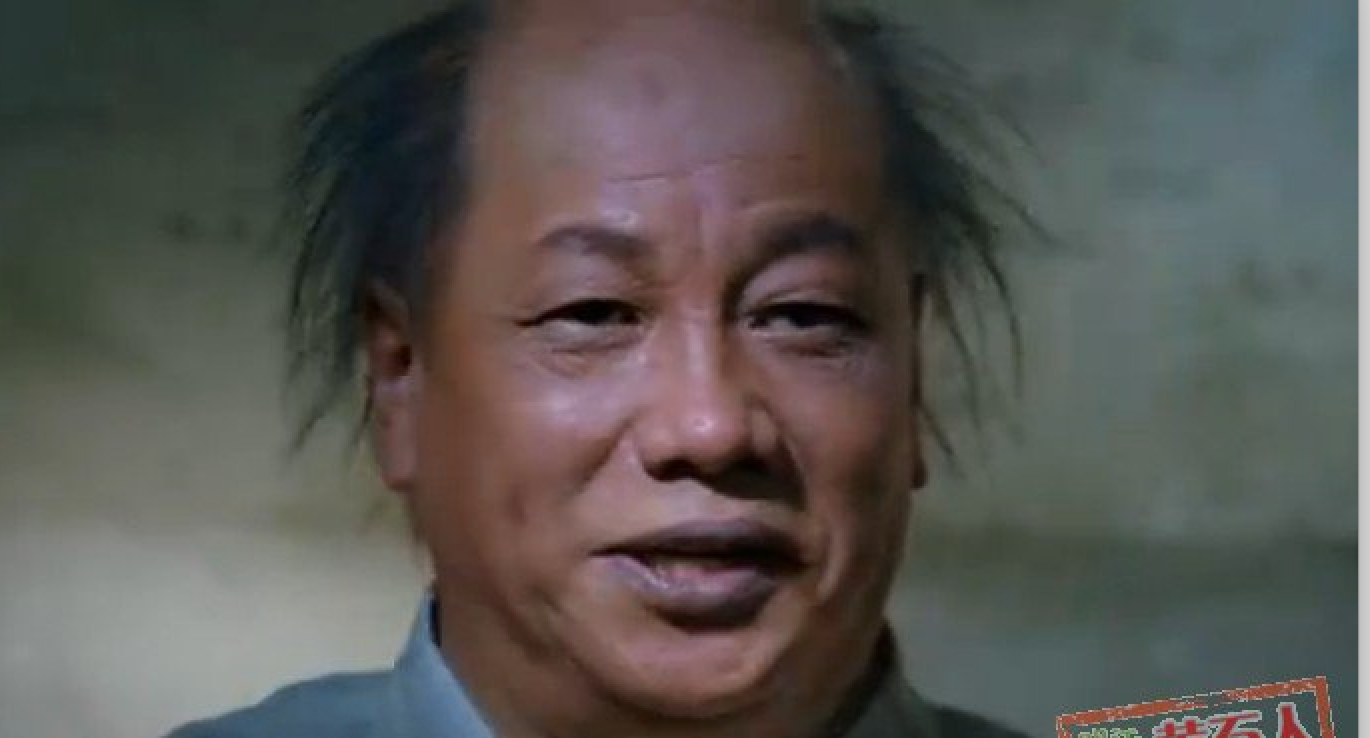
\includegraphics[width=.4\textwidth]{image/source.png}
\hspace{1cm}
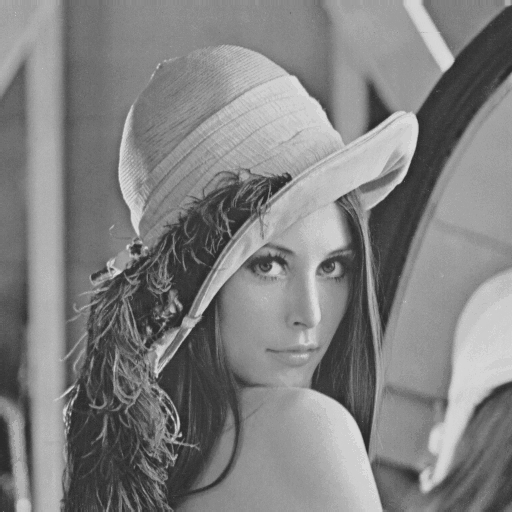
\includegraphics[width=.4\textwidth]{image/gray_image.png}
\caption{Source and Gray Image}%整個標籤
\label{要合併的兩張圖}%整個圖形標籤
\end{figure}
}

\newpage % 新一頁
\subsection{程式碼}

{
\begin{lstlisting}[language=Python]

# 取得並儲存灰階照片
def readGrayImage(name):
    grayImage = cv2.imread(name, cv2.IMREAD_GRAYSCALE)
    savePhoto('gray_image', grayImage)
    return grayImage
    
\end{lstlisting}
}

\section{Lapalcian Enhancement}
\subsection{Lapalcian Mask}
{
用Lapalcian Mask二階微分找影像的邊緣
\begin{figure}[ht]
\centering
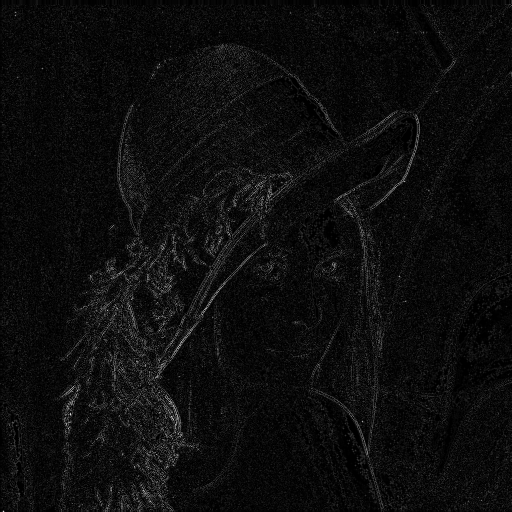
\includegraphics[width=.4\textwidth]{image/laplacian_mask_image.png}
\caption{Lapalcian Mask Edge Image}%整個標籤
\label{要合併的兩張圖}%整個圖形標籤
\end{figure}

程式碼
\begin{lstlisting}[language=Python]
# Lapalcian Mask
def laplacianMask(image):
    lap = cv2.Laplacian(image, cv2.CV_64F)
    lap = np.uint8(np.absolute(lap))
    savePhoto('laplacian_mask_image', lap)
    return lap

\end{lstlisting}
}

\newpage
\subsection{實現Lapalcian Enhancement}
{
把轉成灰階的原始照片與用Lapalcian Mask產生的照片相加
輸出的照片會有雜訊產生
\begin{figure}[ht]
\centering
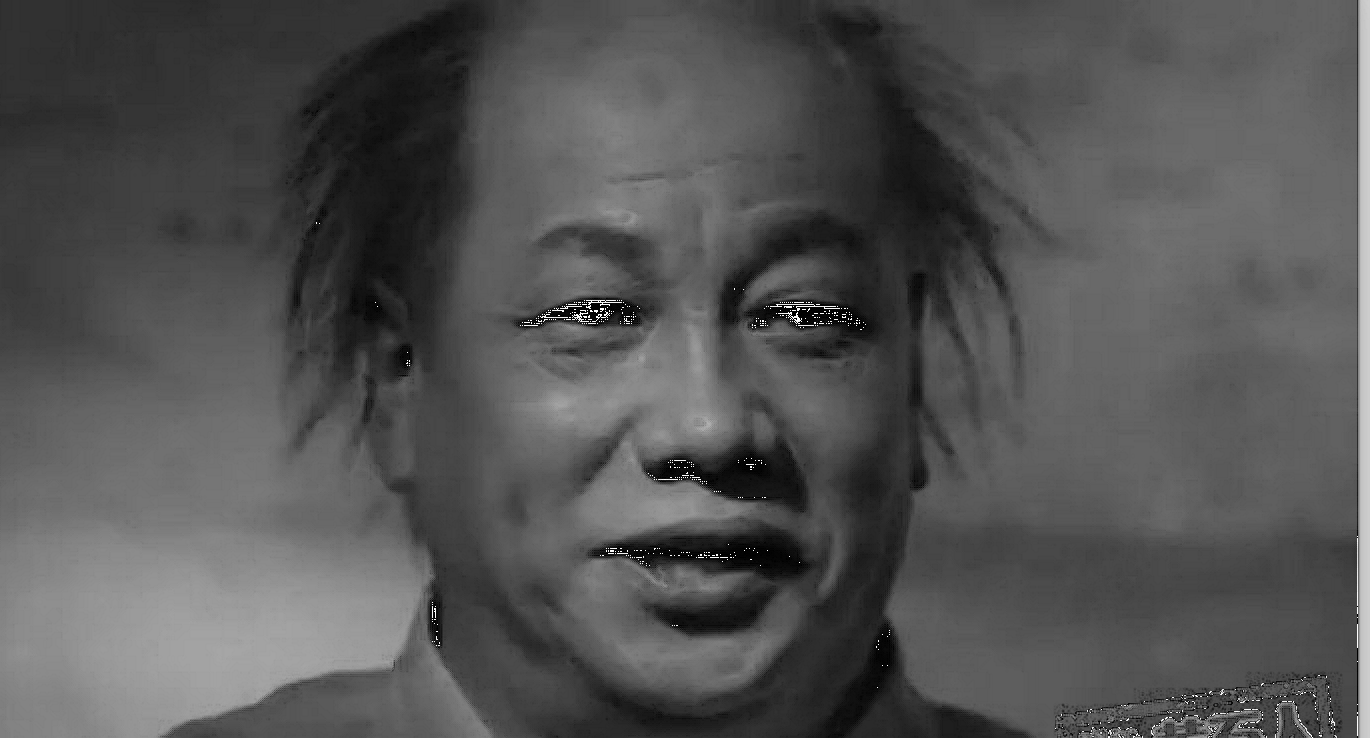
\includegraphics[width=.4\textwidth]{image/lap_enhance_image.png}
\caption{Lapalcian Enhancement Image}%整個標籤
\label{要合併的兩張圖}%整個圖形標籤
\end{figure}


程式碼
\begin{lstlisting}[language=Python]
def lap_enhance(source, lapacian):
    height = source.shape[0]
    width = source.shape[1]
    # height, width, _ = source.shape
    newImage = np.zeros((height, width, 3), np.uint8)
    for x in range(width):
        for y in range(height):
            value = source[y][x] - lapacian[y][x]
            if value > 255:
                value = 255
            else:
                value = int(value)
            newImage[y][x] = value
    savePhoto('lap_enhance_image', newImage)
    return newImage
    
\end{lstlisting}
}

\newpage
\section{Sobel Filter Enhancement}

\subsection{Sobel Filter}
{
利用Sobel Filter找邊緣
\begin{figure}[ht]
\centering
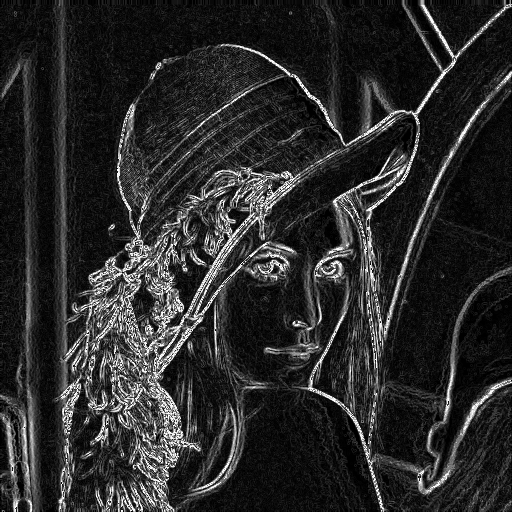
\includegraphics[width=.4\textwidth]{image/sobel_filter_image.png}
\caption{Sobel Filter Image}%整個標籤
\label{要合併的兩張圖}%整個圖形標籤
\end{figure}

程式碼
\begin{lstlisting}[language=Python]
# Sobel Filter
def sobelFilter(image):
    sobelX = cv2.Sobel(image, cv2.CV_64F, 1, 0)
    sobelY = cv2.Sobel(image, cv2.CV_64F, 0, 1)
    sobelX = np.uint8(np.absolute(sobelX))
    sobelY = np.uint8(np.absolute(sobelY))
    sobelCombined = cv2.bitwise_or(sobelX, sobelY)
    savePhoto('sobel_filter_image', sobelCombined)
    
\end{lstlisting}
}

\newpage
\subsection{Convolution}
{
\begin{figure}[ht]
\centering
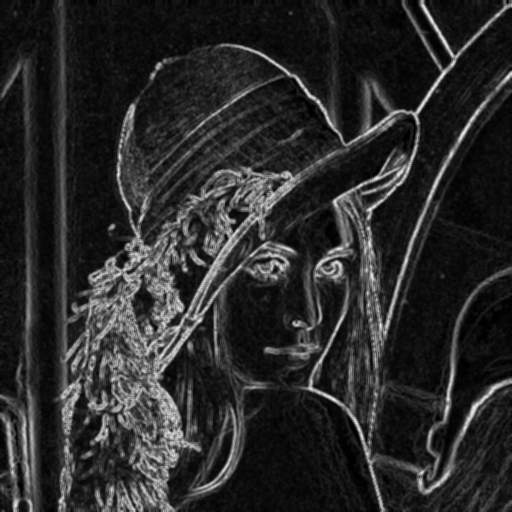
\includegraphics[width=.4\textwidth]{image/convolution_image.png}
\caption{Convolution Image}%整個標籤
\label{要合併的兩張圖}%整個圖形標籤
\end{figure}

程式碼
\begin{lstlisting}[language=Python]
def convolution():
    image = cv2.imread('sobel_filter_image.png')
    blurred = cv2.blur(image, (3, 3))
    savePhoto('convolution_image', blurred)
    return blurred
    
\end{lstlisting}
}

\subsection{Normalization}
{
把影像做正規化,把Convolution模糊化後的影像乘以Lapalcian Mask的影像
\begin{figure}[ht]
\centering
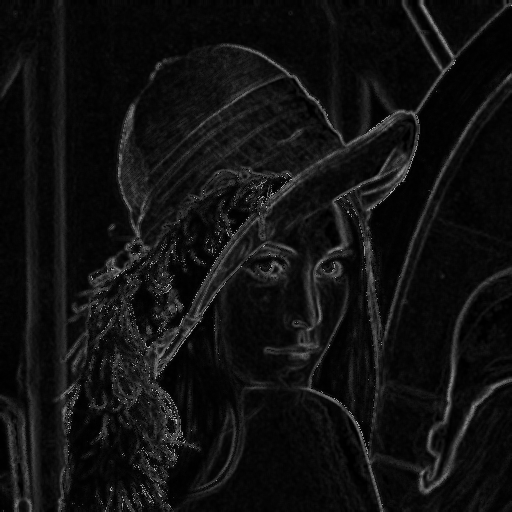
\includegraphics[width=.4\textwidth]{image/normalization_image.png}
\caption{Normalization Image}%整個標籤
\label{要合併的兩張圖}%整個圖形標籤
\end{figure}

程式碼
\begin{lstlisting}[language=Python]
def normalization(source, blur):
    height = source.shape[0]
    width = source.shape[1]
    # height, width, _ = source.shape
    newImage = np.zeros((height, width, 3), np.uint8)
    for x in range(width):
        for y in range(height):
            newImage[y][x] = blur[y][x] / 255 * source[y][x]
    savePhoto('normalization_image', newImage)
    return newImage
    
\end{lstlisting}
}

\subsection{Output}
{
最後把正規化後的影像與原始照片相加,即可產生銳化的影像
\begin{figure}[ht]
\centering
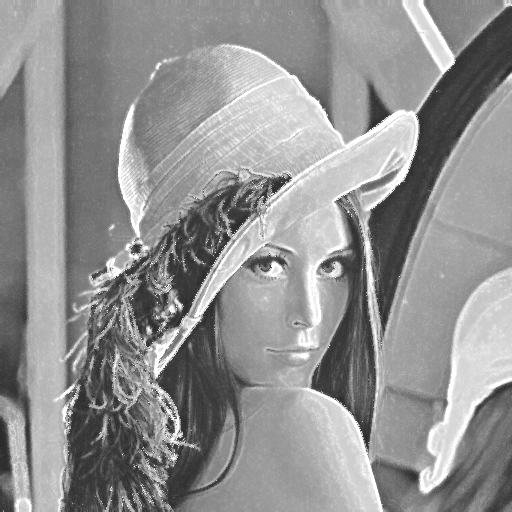
\includegraphics[width=.4\textwidth]{image/FinalEnhancementImage.png}
\caption{Final EnhancementImage Image}%整個標籤
\label{要合併的兩張圖}%整個圖形標籤
\end{figure}

程式碼
\begin{lstlisting}[language=Python]
def enhancementImage_New(source, normalization):
    height = source.shape[0]
    width = source.shape[1]
    # height, width, _ = source.shape
    newImage = np.zeros((height, width, 3), np.uint8)
    for x in range(width):
        for y in range(height):
            tmp2 = int(normalization[y][x][0])
            tmp1 = int(source[y][x])
            tmp0 = tmp1 + tmp2
            print(y, x)
            if tmp0 > 255:
                newImage[y][x] = [255, 255, 255]
            else:
                newImage[y][x] = normalization[y][x] + source[y][x]

            savePhoto('FinalEnhancementImage', newImage)
    
\end{lstlisting}
}

\section{結論}
使用Laplacian Enhancement還是會有雜訊。
\newline
使用Sobel Filter Enhancement雜訊明顯比Laplacian少很多,而且還可以把影像銳化。
\newline
另外在coding時有發現兩張照片像素相加如果超過255時,python會自動減掉255,造成一開始輸出的影像都還是很多雜訊。
\begin{figure}[ht]
\centering
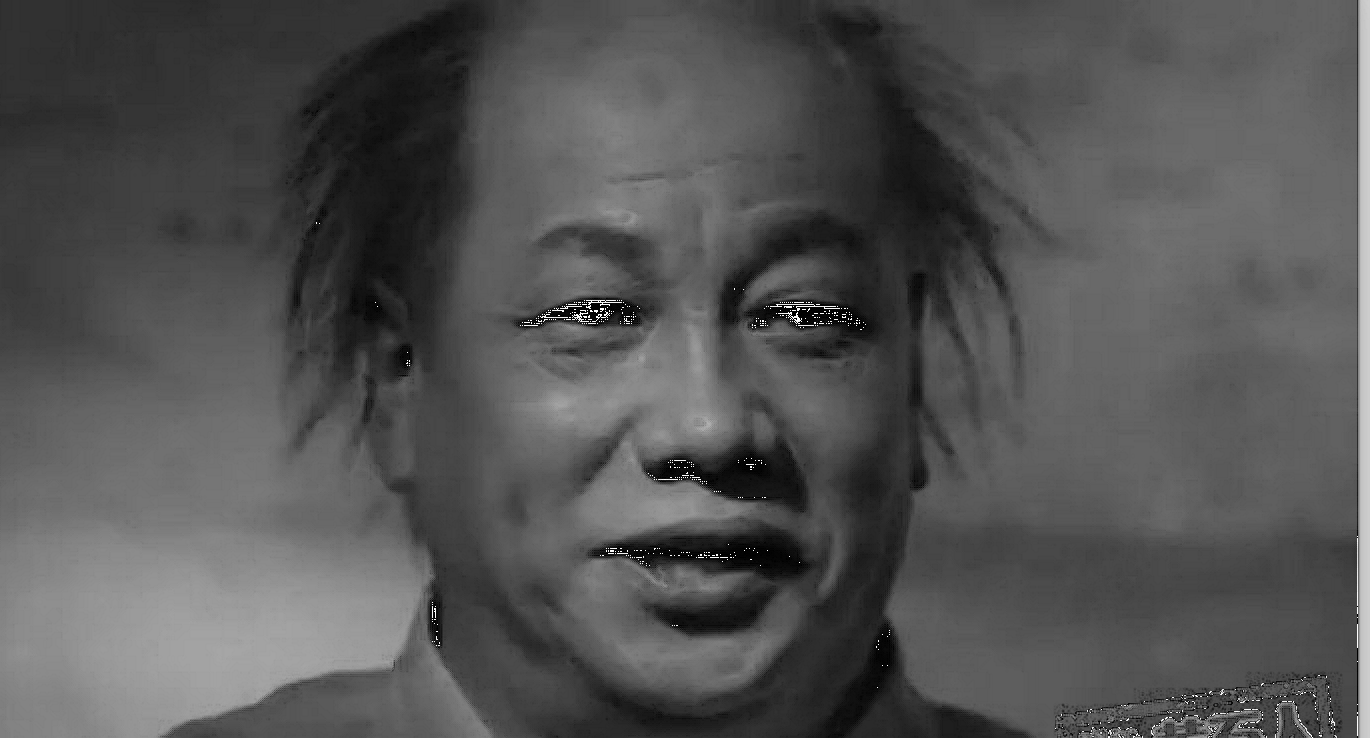
\includegraphics[width=.4\textwidth]{image/lap_enhance_image.png}
\hspace{1cm}
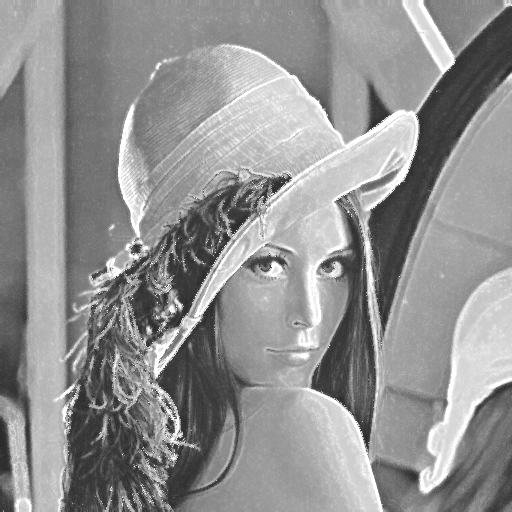
\includegraphics[width=.4\textwidth]{image/FinalEnhancementImage.png}
\caption{Laplacian and Sobel Enhancement Image}%整個標籤
\label{要合併的兩張圖}%整個圖形標籤
\end{figure}
\end{document}